
In the last chapter we have encountered how the VSC$^\pp$-problem becomes tractable for \onewriter{} programs with a complexity $\mathcal{O}(n^{\pp + 1} \cdot k \cdot \pp \cdot \pp!)$. Here are two observations about this complexity: the exponent on $k$ is a constant, whereas the exponent on $n$ is the parameter $\pp$. We remark that to achieve the polynomial-time complexity, we had restricted to \onewriter{}  programs and also assumed that the parameter $\pp$ is fixed. 

Our goal in this chapter is to investigate what happens when we perturb these restrictions. Figure~\ref{fig:results-overview} presents an overview of the complexity results.

\begin{figure}[h]
\centering
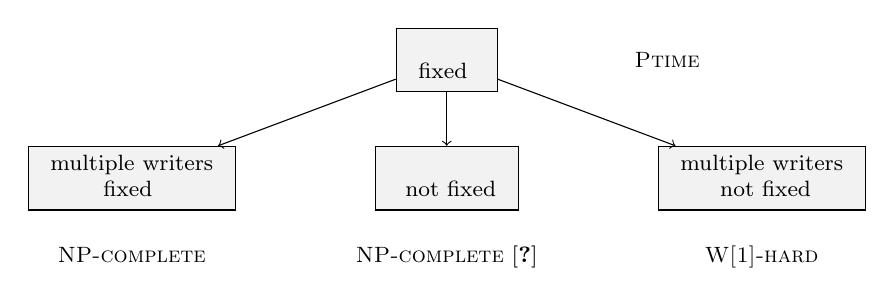
\begin{tikzpicture}[box/.style={rectangle, fill=gray!10, draw, inner sep=2pt}]
  \node[box] (a) at (0,0) {\footnotesize \begin{tabular}{c} \onewriter \\ fixed $\pp$ \end{tabular}};
  \node[box] (b) at (-4,-1.5) {\footnotesize \begin{tabular}{c} multiple writers \\ fixed $\pp$ \end{tabular}};
  \node[box] (c) at (0, -1.5) {\footnotesize \begin{tabular}{c} \onewriter \\ $\pp$ not fixed \end{tabular}};
  \node[box] (d) at (4, -1.5) {\footnotesize \begin{tabular}{c} multiple writers \\ $\pp$ not fixed \end{tabular}};
  
  \begin{scope}[->]
    \draw (a) to (b);
    \draw (a) to (c);
    \draw (a) to (d);
  \end{scope}
 
  \node at (2.8, 0) {\footnotesize \textsc{Ptime} };
  \node at (-4, -2.5) {\footnotesize \begin{tabular}{c} \textsc{NP-complete}  \\  \end{tabular}};
  \node at (0, -2.5) {\footnotesize \textsc{NP-complete}~\cite{gibbons}};
  \node at (4, -2.5) {\footnotesize \begin{tabular}{c} \textsc{W[1]-hard} \\ \end{tabular}}; 
\end{tikzpicture}
\caption{Illustration of the various complexity results}
\label{fig:results-overview}
\end{figure}

We shall discuss the complexity results when multiple writer programs are involved and what happens when $\pp$ is an input parameter. 

\paragraph*{Multiple writers, fixed $\pp$.} When multiple writers are allowed, \vscp\ becomes $\np$-complete, even with \twowriter\ programs (Theorem~\ref{th:NPhardness}). Furthermore, under the Exponential-Time-Hypothesis~\cite{ImpagliazzoPZ01}, we prove that VSC$^\pp$ cannot have a $2^{o(k)} \cdot n^{\mathcal{O}(1)}$ algorithm, even for $0$ preemptions and \threewriter\ programs (Theorem~\ref{th:Finegrained}). Contrast this with \onewriter\ where the exponent on $k$ was a constant $1$, thanks to the conflict analysis. Our hardness results therefore give strong evidence that the presence of multiple writers may introduce an unavoidable exponential on the number of threads $k$. 

\paragraph*{One writer, $\pp$ not fixed.} Now, if we continue with \onewriter\ but assume that $\pp$ is also part of the instance input, then Theorem~4.3 of \cite{gibbons} shows $\NP$-completeness. In their proof, an instance of 3-CNF-SAT with $k$ variables and $m$ clauses is reduced to a \onewriter\ program, where $\pp$ can be taken to be $\mathcal{O}(m + k)$. This is sufficient to prove $\NP$-hardness, when $\pp$ is not fixed. This hardness result provides evidence that having either $n^\pp$ or $k^\pp$ or some exponential function with $\pp$ could be unavoidable -- in our algorithm for Section~\ref{sec:one-writer}, we have $n^\pp$ and $\pp!$ in the running time. 

\paragraph*{Multiple writers, $\pp$ not fixed.} Finally, when we consider multiple writers, and do not fix $\pp$, we show W[1]-hardness (Section~\ref{sec:w1-hard}). W[1] is a complexity class studied in parameterized complexity, which intuitively provides evidence that we cannot have an algorithm with running time $f(\pp) \cdot (k + n)^{\mathcal{O}(1)}$ for our problem when multiple writers are allowed. In other words, we cannot separate out the influence of $\pp$ from $n$ and $k$. In contrast, consider the standard \emph{vertex cover} problem for graphs: given a graph of size $n$ is there a vertex cover of size $\le k$? This is an $\NP$-complete problem, but it has an algorithm of the form $f(k) \cdot n^{\mathcal{O}(1)}$ and hence is called fixed-parameter-tractable (FPT). On the other hand, deciding whether a graph of size $n$ has an \emph{independent set} of size $\ge k$ is known to be W[1]-hard (hence unlikely to be FPT). In Section~\ref{sec:w1-hard}, we reduce the independent set problem to our VSC problem, where the $k$ of the independent set translates to the $\pp$ of our VSC problem. We refer the reader to~\cite{DowneyFellows1999} for an exposition of parameterized complexity classes.

We divide the chapter into three sections. In the firts  begin by showing hardness result for \twowriter{}. The following section gives a lower bound result for \threewriter{} programs assuming ETH. In the last section of this chapter we shall show how the complexity of VSC$^\pp$ becomes \textsc{W[1]}-hard when $\pp$ is a parameter of the problem and not fixed. The results from this chapter are the following

\begin{restatable}{theorem}{scFinegrained}\label{th:Finegrained}
Under ETH, there is no $2^{o(k)} \cdot n^{\mathcal{O}(1)}$ algorithm for \vscp where $k$ is the number of threads, $n$ is the total number of operations.

The result holds even when the input instance is a \threewriter\ program.
\end{restatable}

\begin{restatable}{theorem}{scFinegrained}\label{th:NPhardness}
\vscp is $\NP$-complete, for all $\pi \ge 0$. Hardness holds even for \twowriter\ programs. 
\end{restatable}

\begin{restatable}{theorem}{wonehardness}\label{thm:w1-hard}
When $\pp$ is not fixed, and is treated as a parameter in the input, the \vscp\ problem is W[1]-hard.
\end{restatable} 
We now move on to present the hardness results. Firstly, we note that \vscp\ is in $\NP$, since we can guess an interleaving and check sequential consistency and the preemption bound $\pp$ in linear time. 
We present two hardness results for the case of fixed $\pp$. To show hardness, we provide reductions from 3-CNF-SAT. Given a Boolean formula $\varphi$ over variables $x_1, \dots, x_k$ and clauses $C_1, \dots, C_m$, where each clause is a disjunction of three literals, we ask whether $\varphi$ admits a satisfying assignment. We will start with the reduction to \threewriter\ systems and then adapt the reduction to \twowriter\ systems. The constructions for both the reductions are adapted from Theorem 2.1 of~\cite{Gibbons}. Let us first recall the Exponential Time Hypothesis that we make use of, to deduce a conditional lower bound.



\textbf{Exponential Time Hypothesis (ETH).}~\cite{ImpagliazzoPZ01}
There is no $2^{o(k)}\cdot (k+m)^{\mathcal{O}(1)}$ algorithm for 3-CNF-SAT, where $k$ is the number of variables and $m$ is the number of clauses.



For the reduction to $\threewriter$, we construct a concurrent program consisting of $\mathcal{O}(k)$ threads, i.e., linear in the number of variables of the 3-CNF-SAT instance, and no dependence on the number of clauses $m$. This yields a parameterized reduction and implies the desired conditional lower bound under ETH. In contrast, the reduction to $\twowriter$ uses $\mathcal{O}(k+m)$ threads and is therefore, not a parameterized reduction. Sections~\ref{sec:finegrained} and~\ref{sec:np} describe these reductions in detail.

\paragraph{Notation.}
Let $\varphi$ be a 3-CNF formula over variables $x_1, \dots, x_k$ and clauses $C_1, \dots, C_m$. Each clause $C_j$ consists of three literals $(\ell_j^1, \ell_j^2, \ell_j^3)$, where each literal is either a variable $x_i$ or its negation $\neg x_i$.

For each variable $x_i$, define:
\[
S_{x_i} := \{ j \mid C_j \text{ contains } x_i \}, \qquad
S_{\neg x_i} := \{ j \mid C_j \text{ contains } \neg x_i \}.
\]

Note that for ease of presentation, we omit thread identifiers in events when they are clear from the context.


\section{Fine-grained Hardness under ETH for \threewriter}\label{sec:finegrained}

Given a 3-CNF-SAT instance $\varphi$ in $k$ variable and $m$ clauses, we  construct a \vscp~ instance $\program$ in $\mathcal{O}(k)$ threads and $\mathcal{O}(k+m)$ operations, in $\mathcal{O}(k + m)$ time, such that for every variable only three threads write to it. Therefore, a $2^{o(k)} \cdot n^{\mathcal{O}(1)}$ algorithm for \vscp\ would contradict ETH.
 
\scFinegrained*


Say $\varphi=C_1\land C_2\land \dots \land C_m$. 
The construction for the reduction from $\varphi$, illustrated in Table~\ref{tab:reduction-threads-scmm} shows a program $\program_{\varphi}$ with $6k+1$ threads and $k+m+1$ variables. Variables $v_i, i=1,2,\dots,k$ correspond to $k$ variables of $\varphi$ while variables $c_i, i=1,2,\dots m$ correspond to the clauses. The variable $x$ is a guard to ensure all clause variables $c_i$ are set. Variable $x$ is written only once in $S_f$ while threads writing to $v_i$ are $S_i^0$ and $S_i^1$. Variable $c_i$ is written by $S_{x_i}$ if the clause $C_i$ contains $x$. If clause $C_i$ contains $\neg v_i$, then $c_i$ is written by $S_{\neg x_i}$. As a clause can have at most 3 literals in a 3-CNF-SAT instance, each $c_i$ will be written by at most 3 threads (hence we get a \threewriter\ program). We also pick $\pp$ to be $0$.

\begin{table}[h]
    \caption{Threads in the reduction to \threewriter\ programs}
    \label{tab:reduction-threads-scmm}
    \noindent
    \begin{minipage}{0.38\textwidth}
    \centering
    \begin{tabular}{c | c | c | c}
        $S_i^0$ & $H_i^0$ & $S_i^1$ & $H_i^1$ \\
        $\wt(v_i, 0)$ & $\rd(x, 1)$ & $\wt(v_i, 1)$ & $\rd(x, 1)$ \\
        & $\rd(v_i, 0)$ & & $\rd(v_i, 1)$ 
    \end{tabular}
    \end{minipage}
    \hfill
    \begin{minipage}{0.32\textwidth}
    \centering
    \begin{tabular}{c | c }
        $S_{x_i}$ & $S_{\neg x_i}$ \\
        $\rd(v_i, 1)$ & $\rd(v_i, 0)$ \\
        $\wt(c_j, 1)$ & $\wt(c_j, 1)$ \\
        $\forall j \in C_{x_i}$ & $\forall j \in C_{\neg x_i}$ 
    \end{tabular}
    \end{minipage}
    \hfill
    \begin{minipage}{0.22\textwidth}
    \centering
    \begin{tabular}{c}
        $S_f$ \\
        $\rd(c_1, 1)$ \\
        $\cdots$ \\
        $\rd(c_m, 1)$ \\
        $\wt(x, 1)$
    \end{tabular}
    \end{minipage}
\end{table}

Here is the main idea. In any (complete) $0$-preemption interleaving of $\program_\varphi$, the \emph{helper} threads $H_i^0$ and $H_i^1$ can be executed only after $S_f$ (due to the read-write on variable $x$). This ensures that only one of $S_i^0$ or $S_i^1$ can be executed before $S_f$: otherwise, if both are executed above $S_f$, only the helper thread corresponding to the last write on $v_i$ can be executed after $S_f$. Therefore, since a unique thread between $S_i^0$ or $S_i^1$ appears before $S_f$, we obtain an assignment for the variables. Moreover, as all the clauses have been set to true (thanks to $\rd(c_i, 1)$ in $S_f$), we can conclude that the assignment is satisfying. This leads to the following lemma.

\begin{restatable}{lemma}{threeWriterLemma}\label{lem:eth-sc}
    $\varphi$ is satisfiable iff there exists a sequentially consistent partial interleaving $\sigma$ of $\program_\varphi$ with $0$ preemptions.
\end{restatable}

\begin{proof}
    ($\Rightarrow$)
    Suppose $A$ is a satisfying assignment for $\varphi$. We construct a partial interleaving $\sigma$ as follows. Note that since we want $\sigma$ to have $0$ preemptions, each thread appears as a contiguous block.

    First, for each variable $x_i$, add the events of the thread $S^{A(x_i)}$, in some arbitrary order over $i$. 
    Next, for each $i$, add the thread $S_{x_i}$ if $A(x_i)=1$, and include $S_{\neg x_i}$ if $A(x_i)=0$. 
%    Note that since $\sigma$ has $0$ preemptions, each thread appears as a contiguous block.
%   Again, these threads are appended as contiguous blocks in $\sigma$.
    Since $A$ satisfies $\varphi$, for every clause $C_j$, at least one of the above threads writes $\wt(c_j,1)$ before any read of $c_j$ occurs (see Table~\ref{tab:reduction-threads-scmm}).
    Now add the thread $S_f$ to the interleaving. 
    By construction, for each read $\rd(c_j,1)$ in $S_f$, there is a preceding write $\wt(c_j,1)$ in $\sigma$ with no intervening conflicting write. Therefore, these reads respect the $\scmm$ semantics. The final write $\wt(x,1)$ in $S_f$ ensures that subsequent reads on $x$ read the value $1$.

    Next, for each $i$, add the helper thread $H_i^{A(x_i)}$. 
    Each such thread contains a read $\rd(x,1)$, which reads the value written by the write $\wt(x,1)$ in $S_f$, and a read $\rd(v_i, A(x_i))$, which reads the value written by  the earlier write in $S_i^{A(x_i)}$.
    Finally, add the remaining threads: for each $i$, include $S_i^{\neg A(x_i)}$, $H_i^{\neg A(x_i)}$, and the literal thread corresponding to the negation of $A(x_i)$. All reads in these threads reads the value written by earlier writes in $\sigma$.

    By construction, every read in $\sigma$ has the value written by the most recent preceding write to the same variable with the same value. Hence, $\sigma$ is sequentially consistent. Further, since each thread appears as a contiguous block, $\sigma$ has $0$ preemptions.

    ($\Leftarrow$) Suppose there exists a sequentially consistent partial interleaving $\sigma$ of $\program_\varphi$ with $0$ preemptions.
    Since $\sigma$ has $0$ preemptions, $\sigma$ is essentially just a concatenation of the threads in some order. 

    Each helper thread $H_i^0$ and $H_i^1$ contains a read $\rd(x,1)$, and hence must appear after the write $\wt(x,1)$ in $S_f$.

    Consider a variable $x_i$. If both $S_i^0$ and $S_i^1$ appear before $S_f$ in $\sigma$, then both $\wt(v_i,0)$ and $\wt(v_i,1)$ occur before $S_f$. Since no further writes to $v_i$ occur before the helper threads, only one of the reads $\rd(v_i,0)$ or $\rd(v_i,1)$ can have a preceding matching write with no intervening conflicting write. Thus, at most one of $H_i^0$ or $H_i^1$ can appear after $S_f$, contradicting completeness of $\sigma$. Hence, for each $i$, at most one of $S_i^0$ or $S_i^1$ appears before $S_f$.

From the construction of $\sigma$, we obtain the following assignment
\[
A(x_i) =
\begin{cases}
0 & \text{if } S_i^0 \text{ appears before } S_f \text{ in } \sigma,\\
1 & \text{otherwise.}
\end{cases}
\]
Now consider any clause $C_j$. The read $\rd(c_j,1)$ in $S_f$ requires a preceding write $\wt(c_j,1)$ in $\sigma$ with no intervening conflicting write. Such a write can only come from a thread corresponding to a literal of $C_j$ scheduled before $S_f$. By definition of $A$, this literal evaluates to true. Thus, each clause of $\varphi$ is satisfied.
\end{proof}



\section{NP-Hardness for \twowriter}\label{sec:np}

Here, our objective is to prove hardness even when at most two threads write to each variable. We reduce 3-CNF-SAT to \vscp\ for \twowriter\ programs. In this reduction, a formula $\varphi$ with $k$ variables and $m$ clauses yields a program $\program_\varphi$ with $\mathcal{O}(k+m)$ threads. While this suffices to show $\NP$-hardness, it does not yield the stronger ETH-based lower bound, which requires $\mathcal{O}(k)$ threads (and that does not depend on the number of clauses $m$).


The key challenge here is to reduce the number of threads writing to each clause variable $c_j$ from three (one for each literal in the clause) to at most two, while still encoding the satisfiability of the 3-CNF formula.
For each clause $C_j = (\ell_j^1 \vee \ell_j^2 \vee \ell_j^3)$, we introduce an additional auxiliary variable $d_j$, and modify the construction as follows.

\begin{itemize}[left=0.5em]
\item In the thread corresponding to the third literal $\ell_j^3$, replace the write $\wt(c_j,1)$ with $\wt(d_j,1)$.
\item Introduce a new thread with two events as follows:
\[
S_j = (j : \rd(c_j,1)) \cdot (j : \wt(d_j,1)).
\]
\item In the thread $S_f$, replace each $\rd(c_j,1)$ with $\rd(d_j,1)$.
\end{itemize}

This results in the same outcome. Either clause $C_j$ is set to true due to the third literal (and hence $\wt(d_j, 1)$ happens), or if it needs to be true due to the first or second literal, then $S_j$ comes into effect and performs $\wt(d_j, 1)$.
Let $\program_\varphi$ denote the resulting program. Note that due to the additional threads $S_j$, the total number of threads now also depends on $m$, the number of clauses. 


\begin{restatable}{lemma}{twoWriterLemma}\label{lem:np-two-writer}
$\varphi$ is satisfiable iff there exists a sequentially consistent partial interleaving $\sigma$ of $\program_\varphi$ with $0$ preemptions.
\end{restatable}

\begin{proof}
    The proof follows the same structure as Lemma~\ref{lem:eth-sc}.

    ($\Rightarrow$) Suppose that $A$ is a satisfying assignment for $\varphi$. We construct a partial interleaving $\sigma$ with $0$ preemptions.
    For each variable $x_i$, add the thread $S_i^{A(x_i)}$ and the corresponding literal thread ($S_{x_i}$ if $A(x_i)=1$, otherwise $S_{\neg x_i}$).

    Now, consider a clause $C_j$. If the third literal $\ell_j^3$ is true under $A$, include the thread corresponding to $\ell_j^3$ before $S_f$. Then the write $\wt(d_j,1)$ appears before $S_f$, and the read $\rd(d_j,1)$ in $S_f$ is satisfied.
    Otherwise, one of $\ell_j^1$ or $\ell_j^2$ is true. 
    Include the corresponding literal thread (which writes $\wt(c_j,1)$), followed by $S_j$. Then the read $\rd(c_j,1)$ in $S_j$ has a preceding write with no intervening conflicting write, and $\wt(d_j,1)$ in $S_j$ appears before $S_f$.
    After handling all clauses, add the thread $S_f$. Finally, add all remaining threads. By construction, each read has a preceding matching write with no intervening conflicting write, and $\sigma$ has $0$ preemptions.

\medskip

    ($\Leftarrow$) Suppose there exists a sequentially consistent partial interleaving $\sigma$ with $0$ preemptions. Then $\sigma$ is a concatenation of threads. As in Lemma~\ref{lem:eth-sc}, for each variable $x_i$, at most one of $S_i^0$ or $S_i^1$ appears before $S_f$. Define
\[
A(x_i) =
\begin{cases}
0 & \text{if } S_{i}^0 \text{ appears before } S_f,\\
1 & \text{otherwise.}
\end{cases}
\]

    Consider a clause $C_j$. The read $\rd(d_j,1)$ in $S_f$ must have a preceding write $\wt(d_j,1)$ in $\sigma$ with no intervening conflicting writes. This write can either copme from the thread corresponding to $\ell_j^3$, or from $S_{j}$. If it comes from the thread for $\ell_j^3$, then that thread appears before $S_f$, and hence $\ell_j^3$ evaluates to true under $A$.
    Otherwise, it comes from $S_{j}$. In this case, the read $\rd(c_j,1)$ in $S_{j}$ must have a preceding write $\wt(c_j,1)$ in a literal thread corresponding to $\ell_j^1$ or $\ell_j^2$ that appears before $S_{j}$, and hence before $S_f$. The corresponding literal is therefore true under $A$.

    Thus, in all cases, at least one literal in $C_j$ is true under $A$. Hence $\varphi$ is satisfiable.\qedhere
\end{proof}






Thus, we have shown that the preemption-bounded consistency problem is $\NP$-hard for \twowriter~programs. 



%%%%%%%%%%%%
%%%%%%%%%%%%

\section{W[1]-hardness for VSC$^\pp$ when $\pp$ is an input parameter}\label{sec:w1-hard}


In parameterized complexity, W-hierarchy is a well-known concept. It helps organize parameterized problems according to their level of difficulty. One can refer to  \cite{DowneyFellows1999} for a clear understanding. As discussed earlier, it is believed that $\textsc{FPT} \neq W[1]$. One well known problem in the $W[1]$ class is the $k$-independent set problem.

\textbf{$k$-independent set problem}: Let $G = (V,E)$ be a connected graph with vertex set $V$ and edge set $E$. The $k$-independent set problem asks if there exists a set of vertices $V_k \subseteq V$ of size $k$ such that no two vertices share a common edge.

We will use parameterized reduction to reduce an instance $(G, k)$ of the independent set problem to an instance $(\program_G, \pp)$ with $\pp = 3k$, of the \vscp\ problem and prove the following theorem. 

\wonehardness*


\paragraph*{Construction.} The program $\program_G$ is depicted in Table~\ref{tab:independent-set}. It has an $\Init$ thread, $k$ checker threads $\Checker_1, \Checker_2, \dots, \Checker_k$, and $k$ selector threads $\Sel_1, \Sel_2, \dots, \Sel_k$. There is a variable $y_e$ corresponding to each edge $e \in E$, variables $x_1, x_2, \dots, x_k$ to help pick $k$ vertices, and some book-keeping variables $s, p_0, \dots, p_k$. Figure \ref{fig:Example-w1} may  enhance the understanding of the the construction. The graph at the bottom right of the figure has three vertices \circl{1}, \circl{2} and \circl{3} with edges between \circl{1}, \circl{2} and \circl{2}, \circl{3}. The corresponding edge  varibles are $y_{12}$ and $y_{23}$. We have assumed $k=2$. Hence,  there are two selector threads $S_1$, $S_2$, two checker threads and two variables $x_1$ and $x_2$ to help select a vertex set of size 2 as discussed earlier.



\begin{figure}[!htbp]
    %\begin{wrapfigure}[32]{l}{0.5\columnwidth}
        %\resizebox{0.5\columnwidth}{!}{%
        \newcommand{\xdisposition}{0}
        \newcommand{\ydisposition}{0}
        \newcommand{\xtstep}{0.3}
        \newcommand{\ytstep}{0.7}
        \newcommand{\ybias}{-0.3 }
        \newcommand{\xstep}{2}
        \newcommand{\ystep}{-0.6}
        \newcommand{\xtscale}{0.8}
        \def\crossoutopacity{0.3}
        \def \numevents{29}
        \def\scale{0.8}
        \centering
    %    \resizebox{\columnwidth}{!}{%
        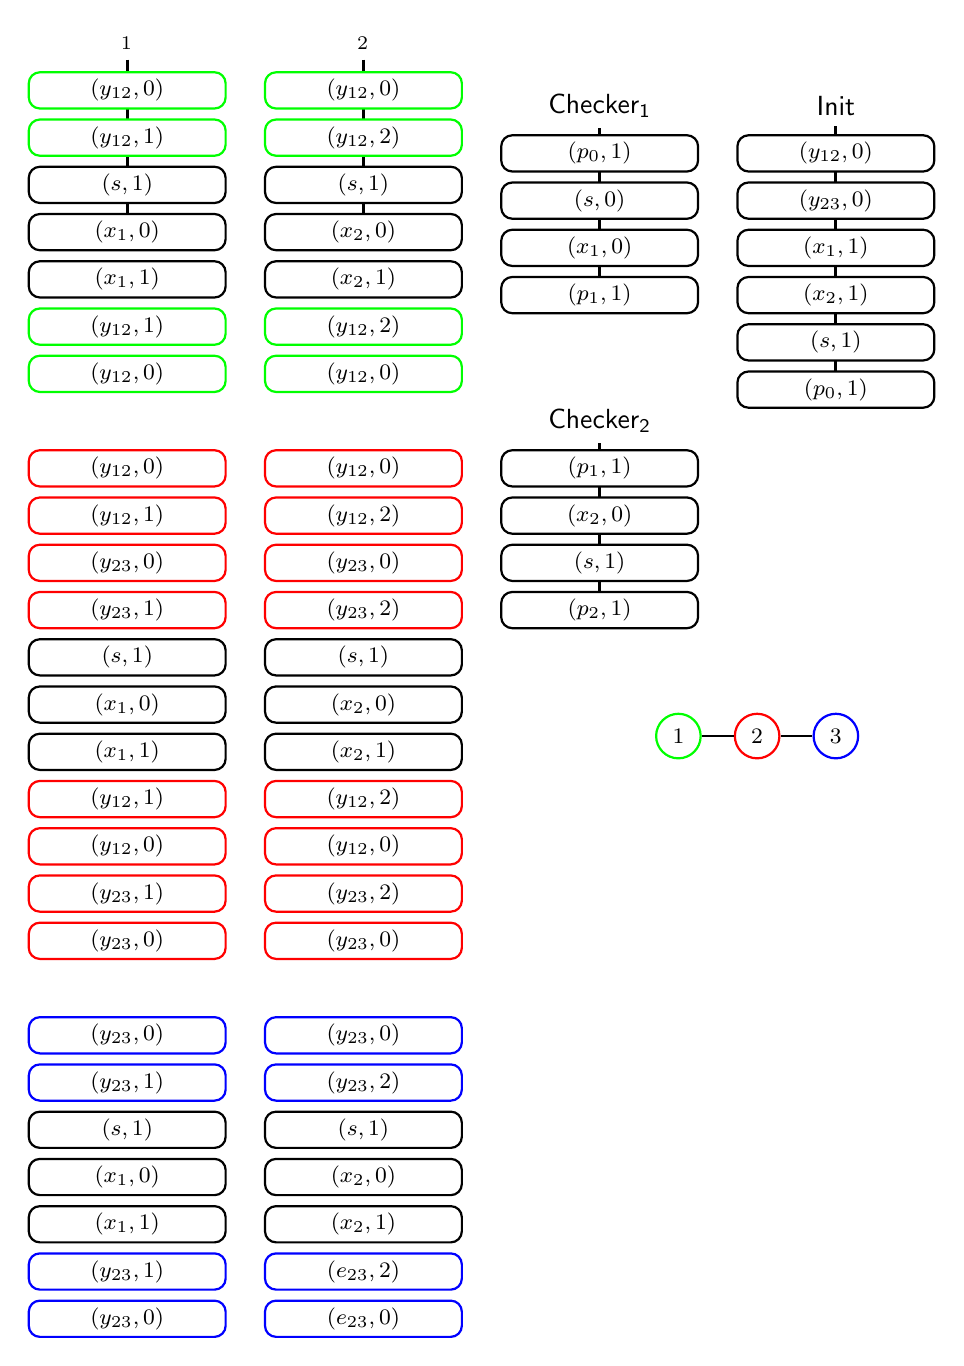
\begin{tikzpicture}[thick, font=\footnotesize,
        pre/.style={<-,shorten >= 2pt, shorten <=2pt, very thick},
        post/.style={->,shorten >= 3pt, shorten <=3pt,   thick},
        seqtrace/.style={line width=1},
        und/.style={very thick, draw=gray},
        virt/.style={circle,draw=black!50,fill=black!20, opacity=0}]
    
        \tikzstyle{event} = [rectangle, fill=white, inner sep=0, minimum height=4.6mm, minimum width=25mm, rounded corners]
    
    
        \node[] (S11) at (.5*\xstep,2*\ystep) {\normalsize $\Sel_{1}$};
        \node[] (S12) at (.5*\xstep,\numevents*\ystep) {};
        \draw[seqtrace] (S11) to (S12);
     
        \node[] (S21) at (2*\xstep,2*\ystep) {\normalsize $\Sel_{2}$};
        \node[] (S22) at (2*\xstep,\numevents*\ystep) {};
        
        
         \draw[seqtrace] (S21) to (S22);
         
    %%%%S1%%%%
       % \node[event, draw=black] (11) at (.5*\xstep, 1*\ystep + 0*\ybias) {$\rd(s, \top)$};
    
        \node[event, draw=green] (12) at (.5*\xstep, 3*\ystep + 0*\ybias) {$\rd(y_{12}, 0)$};
         \node[event, draw=green] (13) at (.5*\xstep, 4*\ystep + 0*\ybias) {$\wt(y_{12}, 1)$};
        
        \node[event, draw=black] (14) at (.5*\xstep, 5*\ystep + 0*\ybias) {$\rd(s, 1)$};
        \node[event, draw=black] (15) at (.5*\xstep, 6*\ystep + 0*\ybias) {$\wt(x_1, 0)$};
        \node[event, draw=black] (16) at (.5*\xstep, 7*\ystep + 0*\ybias) {$\wt(x_1, 1)$};
        
        \node[event, draw=green] (17) at (.5*\xstep, 8*\ystep + 0*\ybias) {$\rd(y_{12},1)$};
        \node[event, draw=green] (18) at (.5*\xstep, 9*\ystep + 0*\ybias) {$\wt(y_{12},0)$};
        
        
    
        \node[event, draw=red] (19) at (.5*\xstep, 11*\ystep + 0*\ybias) {$\rd(y_{12}, 0)$};
        \node[event, draw=red] (20) at (.5*\xstep, 12*\ystep + 0*\ybias) {$\wt(y_{12}, 1)$};
        \node[event, draw=red] (21) at (.5*\xstep, 13*\ystep + 0*\ybias) {$\rd(y_{23}, 0)$};
        \node[event, draw=red] (22) at (.5*\xstep, 14*\ystep + 0*\ybias) {$\wt(y_{23}, 1)$};
        
        
        
        
        
        \node[event, draw=black] (23) at (.5*\xstep, 15*\ystep + 0*\ybias) {$\rd(s, 1)$};
        \node[event, draw=black] (24) at (.5*\xstep, 16*\ystep + 0*\ybias) {$\wt(x_1, 0)$};
        \node[event, draw=black] (25) at (.5*\xstep, 17*\ystep + 0*\ybias) {$\wt(x_1, 1)$};
        
        
        \node[event, draw=red] (26) at (.5*\xstep, 18*\ystep + 0*\ybias) {$\rd(y_{12}, 1)$};
        \node[event, draw=red] (27) at (.5*\xstep, 19*\ystep + 0*\ybias) {$\wt(y_{12}, 0)$};
        \node[event, draw=red] (28) at (.5*\xstep, 20*\ystep + 0*\ybias) {$\rd(y_{23}, 1)$};
        \node[event, draw=red] (29) at (.5*\xstep, 21*\ystep + 0*\ybias) {$\wt(y_{23}, 0)$};
        
        
        
       \node[event, draw=blue] (31) at (.5*\xstep, 23*\ystep + 0*\ybias) {$\rd(y_{23}, 0)$};
        \node[event, draw=blue] (32) at (.5*\xstep, 24*\ystep + 0*\ybias) {$\wt(y_{23}, 1)$};
        \node[event, draw=black] (33) at (.5*\xstep, 25*\ystep + 0*\ybias) {$\rd(s, 1)$};
        \node[event, draw=black] (34) at (.5*\xstep, 26*\ystep + 0*\ybias) {$\wt(x_1, 0)$};
        \node[event, draw=black] (35) at (.5*\xstep, 27*\ystep + 0*\ybias) {$\wt(x_1, 1)$};\node[event, draw=blue] (36) at (.5*\xstep, 28*\ystep + 0*\ybias) {$\rd(y_{23}, 1)$};
        \node[event, draw=blue] (37) at (.5*\xstep, 29*\ystep + 0*\ybias) {$\wt(y_{23}, 0)$};
    
       
    %%%%S2%%%%%
    
    
    % \node[event, draw=black] (11) at (2*\xstep, 1*\ystep + 0*\ybias) {$\rd(s, \top)$};
    
        \node[event, draw=green] (12) at (2*\xstep, 3*\ystep + 0*\ybias) {$\rd(y_{12}, 0)$};
         \node[event, draw=green] (13) at (2*\xstep, 4*\ystep + 0*\ybias) {$\wt(y_{12}, 2)$};
        
        \node[event, draw=black] (14) at (2*\xstep, 5*\ystep + 0*\ybias) {$\rd(s, 1)$};
        \node[event, draw=black] (15) at (2*\xstep, 6*\ystep + 0*\ybias) {$\wt(x_2, 0)$};
        \node[event, draw=black] (16) at (2*\xstep, 7*\ystep + 0*\ybias) {$\wt(x_2, 1)$};
        
        \node[event, draw=green] (18) at (2*\xstep, 8*\ystep + 0*\ybias) {$\rd(y_{12},2)$};
        \node[event, draw=green] (19) at (2*\xstep, 9*\ystep + 0*\ybias) {$\wt(y_{12},0)$};
    
        \node[event, draw=red] (19) at (2*\xstep, 11*\ystep + 0*\ybias) {$\rd(y_{12}, 0)$};
        \node[event, draw=red] (20) at (2*\xstep, 12*\ystep + 0*\ybias) {$\wt(y_{12}, 2)$};
        
        \node[event, draw=red] (21) at (2*\xstep, 13*\ystep + 0*\ybias) {$\rd(y_{23}, 0)$};
       
        \node[event, draw=red] (22) at (2*\xstep, 14*\ystep + 0*\ybias) {$\wt(y_{23}, 2)$};
        
        \node[event, draw=black] (23) at (2*\xstep, 15*\ystep + 0*\ybias) {$\rd(s, 1)$};
        \node[event, draw=black] (24) at (2*\xstep, 16*\ystep + 0*\ybias) {$\wt(x_2, 0)$};
        \node[event, draw=black] (25) at (2*\xstep, 17*\ystep + 0*\ybias) {$\wt(x_2, 1)$};
        
        
        \node[event, draw=red] (26) at (2*\xstep, 18*\ystep + 0*\ybias) {$\rd(y_{12}, 2)$};
        \node[event, draw=red] (28) at (2*\xstep, 19*\ystep + 0*\ybias) {$\wt(y_{12}, 0)$};
        \node[event, draw=red] (29) at (2*\xstep, 20*\ystep + 0*\ybias) {$\rd(y_{23}, 2)$};
        \node[event, draw=red] (30) at (2*\xstep, 21*\ystep + 0*\ybias) {$\wt(y_{23}, 0)$};
        
        
       \node[event, draw=blue] (31) at (2*\xstep, 23*\ystep + 0*\ybias) {$\rd(y_{23}, 0)$};
        \node[event, draw=blue] (32) at (2*\xstep, 24*\ystep + 0*\ybias) {$\wt(y_{23}, 2)$};
        \node[event, draw=black] (33) at (2*\xstep, 25*\ystep + 0*\ybias) {$\rd(s, 1)$};
        \node[event, draw=black] (34) at (2*\xstep, 26*\ystep + 0*\ybias) {$\wt(x_2, 0)$};
        \node[event, draw=black] (35) at (2*\xstep, 27*\ystep + 0*\ybias) {$\wt(x_2, 1)$};
         \node[event, draw=blue] (36) at (2*\xstep, 28*\ystep + 0*\ybias) {$\rd(e_{23}, 2)$};
        \node[event, draw=blue] (37) at (2*\xstep, 29*\ystep + 0*\ybias) {$\wt(e_{23}, 0)$};
    
    %%%%%%%%%%%%%%%%%%%%%%%%%%%%%%%%%%%%%%%%%%%%%%%%%%%%%%
            
       
       \def \numevents{4}
      
       \begin{scope}[xshift=0cm,yshift=-2cm]
         
                \node[] (S11) at (3.5*\xstep,0) {\normalsize $\mathsf{Checker_1}$};
                \node[] (S12) at (3.5*\xstep, \numevents* \ystep) {};
            
                \draw[seqtrace] (S11) to (S12);
            
                
                \node[event, draw=black] (11) at (3.5*\xstep, 1*\ystep + 0*\ybias) {$\rd(p_{0}, 1)$};
                \node[event, draw=black] (12) at (3.5*\xstep, 2*\ystep + 0*\ybias) {$\wt(s, 0)$};
                
                \node[event, draw=black] (13) at (3.5*\xstep, 3*\ystep + 0*\ybias) {$\rd(x_1, 0)$};
                \node[event, draw=black] (13) at (3.5*\xstep, 4*\ystep + 0*\ybias) {$\wt(p_1, 1)$};
                
        
        \end{scope}
        
        \begin{scope}[xshift=0cm,yshift=-6cm]
         
                 \node[] (S11) at (3.5*\xstep,0) {\normalsize $\mathsf{Checker_2}$};
                \node[] (S12) at (3.5*\xstep, \numevents* \ystep) {};
            
                \draw[seqtrace] (S11) to (S12);
            
                
                \node[event, draw=black] (11) at (3.5*\xstep, 1*\ystep + 0*\ybias) {$\rd(p_{1}, 1)$};
              \node[event, draw=black] (12) at (3.5*\xstep, 2*\ystep + 0*\ybias) {$\rd(x_2, 0)$};                
                \node[event, draw=black] (13) at (3.5*\xstep, 3*\ystep + 0*\ybias) {$\wt(s, 1)$};                
                \node[event, draw=black] (13) at (3.5*\xstep, 4*\ystep + 0*\ybias) {$\wt(p_2, 1)$};
                
        
        \end{scope}
       
        
        \def \numevents{6}
          \begin{scope}[xshift=3cm,yshift=-2cm]
         
                \node[] (S11) at (3.5*\xstep,0) {\normalsize $\mathsf{Init}$};
                \node[] (S12) at (3.5*\xstep, \numevents* \ystep) {};
            
                \draw[seqtrace] (S11) to (S12);
            
                
                \node[event, draw=black] (11) at (3.5*\xstep, 1*\ystep + 0*\ybias) {$\wt(y_{12}, 0)$};
                \node[event, draw=black] (12) at (3.5*\xstep, 2*\ystep + 0*\ybias) {$\wt(y_{23}, 0)$};
                \node[event, draw=black] (13) at (3.5*\xstep, 3*\ystep + 0*\ybias) {$\wt(x_{1}, 1)$};
                \node[event, draw=black] (14) at (3.5*\xstep, 4*\ystep + 0*\ybias) {$\wt(x_2, 1)$};
                \node[event, draw=black] (15) at (3.5*\xstep, 5*\ystep + 0*\ybias) {$\wt(s, 1)$};
                \node[event, draw=black] (15) at (3.5*\xstep, 6*\ystep + 0*\ybias) {$\wt(p_0, 1)$};
        
        \end{scope}
        
    
                \begin{scope}[xshift=8cm,yshift=-10cm]
                \node[circle, draw=green, minimum size=.3cm] (1) {1};
                \node[circle, draw=red, minimum size=.3cm, right of=1] (2) {2};
                \node[circle, draw=blue, minimum size=.3cm, right of=2] (3) {3};
            
                % Edges
                \draw[-] (1) -- (2);
                \draw[-] (2) -- (3);
                \end{scope}
            
      
        \end{tikzpicture}   
        %}
        %}
        \caption{The $W[1]$-hardness reduction.}
        \label{fig:Example-w1}
    %\end{wrapfigure}
\end{figure}



 

\begin{table}
\centering
\caption{Reduction from $k$-independent set problem. Index $j$ ranges from $1$ to $k$.}
\label{tab:independent-set}
\medskip
\centering
\begin{tabular}{l  @{\qquad} l  @{\qquad} l }
    $\Init$ &  $\Checker_j$ & $~\Sel_j$ \\
    &  & \\
$\wt(y_e, 0)$   &  $\rd(p_{j-1}, 1)$ &   $\forall v \in V:$  \\
$\forall e \in E$  &  $\wt(s, 0)$ when $j \neq k$ &  \\
& & $\rd(y_e, 0);~\wt(y_e, j)$ \quad $\forall e \in E$ containing $v$ \\
$\wt(x_j, 1)$ &  $\rd(x_j, 0)$  &  \\
$\forall 1 \le j \le k$ & $\wt(s, 1)$ when $j = k$  & $\rd(s, 1)$   \\
  & &  $\wt(x_j, 0)$   \\
$\wt(s, 1)$ & $\wt(p_j, 1)$ &  $\wt(x_j, 1)$  \\
$\wt(p_0, 1)$ & &   \\
 & &   $\rd(y_e, j);~\wt(y_e, 0)$ \quad $\forall e \in E$ containing $v$  
\end{tabular}
\end{table}

The $\Init$ thread is self-explanatory from Table~\ref{tab:independent-set}. For the first $k-1$ checker threads $\Checker_j$ (with $1 \le j \le k-1$) the second operation is $\wt(s, 0)$ (depicted as $\wt(s,0)$ when $j \neq k$). These threads do not have a $\wt(s,1)$ instruction at all. For the last checker thread $\Checker_k$, there is no $\wt(s,0)$, and instead there is a $\wt(s, 1)$ right after $\rd(x_j, 0)$. 
with three blocks each corresponding to the three vertices of the given graph
We now explain the selector threads. Each selector thread $\Sel_j$  
has $|V|$ blocks of operations, one block for each $v \in V$. Taking $V = \{u_1, \dots, u_n\}$, the selector thread $\Sel_j$ can be seen as:
\begin{align*}
 \Sel_j: \quad \BB^j_{u_1}~ \BB^j_{u_2}~\cdots~ \BB^j_{u_n}
\end{align*} 
where each $B^j_u$ is a block of operations corresponding to a vertex $u$. This can further be seen as sub-blocks:
\begin{align*}
 \BB^j_u:~~&~  \Start^j_u ~~\rd(s, 1) ~~ \wt(x_j, 0) ~~ \wt(x_j, 1) ~~ \Finish^j_u \\
 \text{ where~} \qquad \qquad \Start^j_u: ~~& ~\rd(y_e, 0) ~ \wt(y_e, j) ~~ \forall e  \text{ incident on } u \\
\Finish^j_u: ~~& ~\rd(y_e, j) ~ \wt(y_e, 0) ~~ \forall e \text{ incident on } u
\end{align*}
Figure~\ref{fig:Example-w1} shows each selector thread with three blocks each, corresponding to the three vertices of the given graph. Example for vertex \circl{1}, $\Sel_1$ has the block 
 $$B_1^1:~\rd(y_{12},0) \wt(y_{12},1) \quad \rd(s,0) \wt(x_1,0) \wt(x_1,1) \quad \rd(y_{12},1) \wt(y_{12},0)$$
 

%%%%%%%%%correctness%%%%%%%%%

The correctness of the construction is explained through the next two lemmas.

\begin{lemma}\label{lem:independent-set-to-SC-interleaving}
If $G$ has an independent set of size $k$, there is an SC interleaving for $\program_G$ with $3k$ preemptions.
\end{lemma}
\begin{proof} 
Suppose $G$ has an independent set $\{v_1, v_2, \dots, v_k\}$ of size $k$. Then $\program_G$ will have $k$ selector threads. 
Consider an SC interleaving of $\program_G$. It begins with the execution of the $\Init$ thread. The checker and selector threads appear later. 
Notice two conflicting events: the $\Init$ thread has $\wt(x_j, 1)$ whereas $\Checker_j$ has a read $\rd(x_j, 0)$. Therefore, a $\wt(x_j, 0)$ has to appear somewhere in between. This can be provided by $\Sel_j$: for $\wt(x_j, 0)$ to be the last write between the conflicting events in $\Init$ and $\Checker_j$, a part of $\Sel_j$ ending at a $\wt(x_j,0)$ operation should appear in between. So, we say that $\Sel_j$ is ``inside'' some block corresponding to a vertex -- call this vertex $v_j$. Intuitively, we require every $\Sel_j$ to have executed upto a $\wt(x_j, 0)$, then wait for $\Checker_j$ to finish, and subequently execute the rest of $\Sel_j$ that starts with $\wt(x_j, 1)$. However, we cannot do this na\"ively. Suppose $\Sel_1$ executes upto $\wt(x_1,0)$ of $\BB^1_{v_1}$. Then at the start of this block, we have writes $\wt(y_e, 1)$ for all $e$ incident on $v_1$. This may disable the execution of $\Sel_2$ -- notice that the beginning of each block contains a read of the form $\rd(y_e, 0)$. Therefore we need to carefully reach to $\wt(x_j, 0)$ in each thread. We do this in phases. 

\begin{figure}[h]
\centering
\scalebox{0.85}{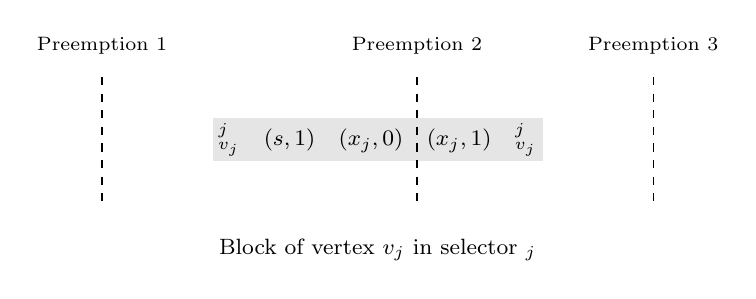
\begin{tikzpicture}[box/.style={rectangle, fill=gray!20, inner sep=2pt}]
\begin{scope}[every node/.style={box}]
  
  \node (b) at (4,0) {\footnotesize $\Start^j_{v_j}~$ $~\rd(s, 1)~$ $~\wt(x_j,0)~$ $~\wt(x_j, 1)~$ $~\Finish^j_{v_j}$ };
\end{scope}
\node at (4, -1.4) {\footnotesize Block of vertex $v_j$ in selector $\Sel_j$};
\draw [dashed] (0.5, 0.8) -- (0.5, -0.8);
\draw [dashed] (4.5, 0.8) -- (4.5, -0.8);
\draw [dashed] (7.5, 0.8) -- (7.5, -0.8);

\node at (0.5, 1.2) {\scriptsize  Preemption $1$};
\node at (4.5, 1.2) {\scriptsize  Preemption $2$};
\node at (7.5, 1.2) {\scriptsize  Preemption $3$};
\end{tikzpicture}}
\caption{Illustrating the preemption points within a selector thread}
\label{fig:w1-illustration}
\end{figure}

%%%%


\begin{description}
\item[Phase 0.] First execute $\Init$ completely.
\item[Phase 1.] We make all the selector threads execute upto the beginning of some block (see preemption $1$ in Figure~\ref{fig:w1-illustration}), one after the other. For example if $v_1=u_m$, execute $\Sel_1$ execute from $\BB^1_{u_1}$ upto $\BB^1_{u_{m-1}}$. Since the end of each block ``resets'' $y_e$ to $0$ (through the $\wt(y_e, 0)$ instruction), such an execution is possible. This phase incurs $k$ preemptions. 

\item[Phase 2.] As a second step, we make every selector $Sel_j$  execute upto $\wt(x_j, 0)$, that is, between preemption points $1$ and $2$ in Figure~\ref{fig:w1-illustration}. The crucial point is that this phase of executions is possible only when the selectors have picked an independent set: on executing $\Sel_j$ upto preemption point $2$, all $y_e$ for edges $e$ incident on $v_j$ have been set to $j$, but since none of these edges is incident on a $v_i$ ($i \neq j$), the selector thread $\Sel_i$ can also pass through its $\rd(y_{e'}, 0)$ operations and execute upto $\wt(x_i, 0)$. Again this phase ends with $k$ preemptions. 

%the $\rd(s,1)$ operation present in block $v_1$, then $\Sel_2$ upto $\rd(s_1)$ in block $v_2$, and so on until $\Sel_k$ upto $\rd(s, 1)$ of block $v_k$. There are $2k$ preemptions so far.
%\item Execute $\Sel_1$ upto $\wt(x_1, 0)$ of block $v_1$. All edges incident on $v_1$ now have a preceding $\wt(y_e, 1)$. Since we started with an independent set, none of these edges are incident on $v_2, \dots, v_k$. Similarly, we can execute $\Sel_2$ upto $\wt(x_2, 0)$, followed by $\Sel_3$, until we finish with $\Sel_k$ upto $\wt(x_k, 0)$. The fact that we started with an independent set allows to parallely execute all the blocks corresponding to $v_1, \dots, v_k$. In this phase, there are $k$ more preemptions.
\item[Phase 3.] Now, we completely execute $\Checker_1$, followed by $\Checker_2$, and so on, until $\Checker_k$. No extra preemptions get added. 
\item[Phase 4.] After all the $k$ checkers are executed, we want to execute the rest of the selector threads after the checker threads are completed. However, executing the full selector may not be possible since some of the $y_e$ variables have current values different from $0$. So to once again reset all $y_e$ to $0$, we execute each selector upto $\wt(y_e, 0)$ at end of the current block. Here we stand at the preemption point $3$ shown in Figure~\ref{fig:w1-illustration}. Total number of preemptions so far is $3k$.

\item[Phase 5. ] Finally, we can execute all the $\Sel_j$ threads one by one without incurring any preemptions. 
\end{description} 

This shows that when the selectors choose an independent set, an SC interleaving with at most $3k$ preemptions is possible, with $3$ preemptions occuring in each selector thread.

Also by construction, the interleaving is sequentially consistent. 
\end{proof}

\begin{lemma}\label{lem:sc-interleaving-to-independent-set}
If $\program_G$ has an SC interleaving, then $G$ has an independent set of size $k$.
\end{lemma}
\begin{proof} 

Suppose there is an SC interleaving of $\program_G$. Here are some observations.
\begin{itemize}
\item Before the $\rd(x_j, 0)$ event of $\Checker_j$, the last write on $x_j$ should be $\wt(x_j, 0)$. Hence $\Sel_j$ should have executed the operations inside some block $\BB^j_{v_j}$ upto $\wt(x_j, 0)$.  
%\item Due to the read $\rd(x_j, 0)$ in $\Checker_j$, the selector thread should be inside a block, and end at $\wt(x_j, 0)$ of some vertex $v_j$, before the $\rd(x_j,0)$.
\item Due to the $p_j$ variables, $\Checker_1$ executes completely before $\Checker_2$. Similarly, $\Checker_2$ executes completely before $\Checker_3$ starts, and so on.
\item Notice the $\wt(s, 0)$ in $\Checker_1$, and a $\rd(s, 1)$ in every block $\BB^j_{v_j}$. Since, (1) all instructions upto $\wt(x_j, 0)$ need to be done before $\Checker_j$, and (2) $\rd(s, 1)$ cannot happen after $\Checker_1$, we deduce that all the selectors have executed atleast upto $\rd(s, 1)$ before the $\wt(s,0)$ of $\Checker_1$. In particular, the block $\Start^j_{v_j}$ is executed before $\wt(s, 0)$ of $\Checker_1$.

%\item Due to the $\wt(s,0)$ in $\Checker_j$, for $j < k$, no selector thread can enter a block between $\Checker_j$ and $\Checker_{j+1}$: that is, the operation $\rd(s,1)$ and the statements above it in every selector should have been executed before $\Checker_1$ begins. 
\end{itemize} 
The crucial point is that: before the $\wt(s,0)$ of $\Checker_1$, we have executed the operation $\wt(y_e, j)$ for all edges incident on $v_j$, due to the block $\Start^j_{v_j}$. We claim that there can be no edge between $v_i$ and $v_j$ when $i \neq j$. Suppose there is an edge $e = (v_i, v_j)$ between two selected vertices. Firstly, when the checkers start executing, all selectors $S_l$ must be inside some block $B^l_{v_l}$. Thread $\Sel_i$ has a $\wt(y_e, i)$ and thread $\Sel_j$ has a $\wt(y_e, j)$ before $\wt(x_i, 0)$ and $\wt(x_j, 0)$ respectively. Notice the reads $\rd(y_e, i)$ in $\Sel_i$ and $\rd(y_e, j)$ in $\Sel_j$ in the $\Finish$ blocks,  which need to be executed, after the $\Checker$ threads. This would not be possible in an SC interleaving. We conclude that there can be no common edge between $v_i$ and $v_j$. This shows that the selected vertices form an independent set, of size $k$. 
\end{proof}

The two lemmas above prove the correctness of our reduction. If $G$ has an independent set of size $k$, we get an interleaving in $\program_G$ with $3k$ preemptions (Lemma~\ref{lem:independent-set-to-SC-interleaving}). If $\program_G$ has an SC interleaving with $3k$ preemptions, in particular, this means there is an SC interleaving. Lemma~\ref{lem:sc-interleaving-to-independent-set} shows there is an independent set of size $k$. 

\section{Discussion}

In the last two chapters, we have studied  the fundamental VSC-problem in the context of bounded preemptions. This is a deviation from the usual parameters
considered in the study of this problem. The results are two-fold: an algorithm
for the single-writer case, and hardness reductions in the presence of multiple
writers, and unbounded preemptions. On the algorithmic front, the key insight is
that for 1-Writer systems the idea of a conflict graph helps to determine order-
ing without having to fall back on a systematic enumeration of all permutations. 
Such a trick is not possible in the case of multiple writers.
In fact the problem seems harder with increase in number of writers. 


Investigating a preemption-bounded version of stateless model-checking under
the reads-value-from equivalence and the impact of incorporating the VSC $\pp$ problem into the procedure, remain directions for future work. Another interesting
direction is to investigate the consistency problem for the Total Store Ordering
(TSO) memory model under the influence of various context-switches \cite{TSO-context-bounding} defined
in the literature.



\endinput










%%%%%%%%%%%%%%%%%%%%%%%%%%%%%%%%%
 




